\documentclass[fleqn,12pt]{article}

\usepackage[utf8]{inputenc}
\usepackage[T1]{fontenc}
\usepackage{mathtools} %loads amsmath
\usepackage{amsthm}
\usepackage{amsfonts}
\usepackage{amsmath}
\usepackage{amssymb}
\usepackage{graphicx}
\usepackage{tikz}
\usetikzlibrary{arrows,automata,positioning}
\usepackage{arydshln}
\usepackage{stmaryrd}
\usetikzlibrary{arrows,automata}
\usepackage{ stmaryrd }

\usepackage{fancyhdr}
\setlength{\headheight}{26pt}
\pagestyle{fancy}
\lhead{Static Program Analysis WS 2016/17 -- Series 05 \\ \small{Igor Dudschenko (296764), Oliver Westphal (358321)}}
\rhead{}

\newcommand\dbrackets[1]{\llbracket #1 \rrbracket}

\setlength{\parindent}{0cm}
\newcommand\note[1]{\textcolor{red}{#1}}

\begin{document}
\section*{Exercise 1}
\subsection*{a)}
\[ \varphi_l(\delta) :=
  \begin{cases}
    \delta       & \quad \text{if } B^l = skip \text{or} B^l \in BExp\\
    \delta [x] \mapsto val_d(a) & \quad \text{if } B^l=(x:=a)\\
  \end{cases}
\]
$$val_{\delta}(x):=\delta (x)$$
$$val_{\delta}(z):=[z,z]$$
$$val_{\delta}(a_1/a_2):=val_{\delta}(a_1) \oslash val_{\delta}(a_2)$$
$$[y_1,y_2] \oslash [z_1,z_2]=
	\begin{cases}
		[-\infty,\infty]\text{, if } 0 \in [z_1,z_2]\\
		[\bigsqcup S,\bigsqcap S] \text{, otherwise}
	\end{cases}$$
where $$S=\{y_1/z_1,y_1/z_2,y_2/z_1,y_2/z_2\}$$
\subsection*{b)}
To show:
$$\text{If: }x_1 \sqsubseteq x_2 \text{ than also } \varphi_l(\delta)(x_1) \sqsubseteq \varphi_l(\delta)(x_2)$$
For:
\[ \varphi_l(\delta) :=
  \begin{cases}
    \delta       & \quad \text{if } B^l = skip \text{ or } B^l \in BExp\\
  \end{cases}
\]
the statement obviously holds.
We have four cases to show for:
\[ \varphi_l(\delta) :=
  \begin{cases}
    \delta [x] \mapsto val_d(a) & \quad \text{if } B^l=(x:=a)\\
  \end{cases}
\]
\begin{itemize}
	\item{$\oplus$ :} $[y_1,y_2] \oplus [z_1,z_2] := [y_1+z_1,y_2+z_2]$ Assume that $y_1 \leq y_2$ and $z_1 \leq z_2$, Proof by Contradiction: Assume there exists a sum, s.t. $y_i \neq y_1 \text{ and } y_1<y_i<y_2$ and $z_j \neq z_1 \text{ and } z_1<z_j<z_2$, such that $y_i+z_i<y_1+z_1$, than the following also holds: $y_i=y_1+a,z_j=z_1+b \text{ with: } a,b\in \mathbb{N}$, but than $y_i+z_i<y_1+z_1$ cannot hold, and therefore $\oplus$ holds and is monotonic. (analogously for: $y_i+z_j<y_2+z_2$)
	\item{$\ominus$ :} $[y_1,y_2] \ominus [z_1,z_2] := [y_1-z_2,y_2-z_1]$ Assume that $y_1 \leq y_2$ and $z_1 \leq z_2$, Proof by Contradiction: Assume there exists a subtraction, s.t. $y_i \neq y_1 \text{ and } y_1<y_i<y_2$ and $z_j \neq z_2 \text{ and } z_1<z_j<z_2$, such that $y_i+z_i<y_1+z_1$, than the following also holds: $y_i=y_1+a,z_j=z_1+b \text{ with: } a,b\in \mathbb{N}$, but than $y_i+z_i<y_1+z_1$ cannot hold, and therefore $\oplus$ holds and is monotonic. (analogously for: $y_i+z_j<y_2+z_2$)
	\item{$\otimes$ :} $[y_1,y_2] \otimes [z_1,z_2]=[\bigsqcap\{y_1/z_1,y_1/z_2,y_2/z_1,y_2/z_2\},\bigsqcup\{y_1/z_1,y_1/z_2,y_2/z_1,y_2/z_2\}]$
	\item{$\oslash$ :} $[y_1,y_2] \oslash [z_1,z_2]=[\bigsqcap\{y_1/z_1,y_1/z_2,y_2/z_1,y_2/z_2\},\bigsqcup\{y_1/z_1,y_1/z_2,y_2/z_1,y_2/z_2\}]$
\end{itemize}

\section*{Exercise 2}

\section*{Exercise 3}
\subsection*{a)}
We define $\sqsubseteq$ as the smallest relation such that\\
\begin{enumerate}
\item $d \sqsubseteq d$, $\forall d \in D$
\item $(n,0) \sqsubseteq \infty$, $\forall n \in \mathbb{N}$
\item $\infty \sqsubseteq (n,1)$, $\forall n \in \mathbb{N}$
\item $(n,s) \sqsubseteq (n',s')$ iff \\ 
	$s < s'$\\
	or $s=s'=0 \wedge n \leq n'$\\
	or $s=s'=1 \wedge n \geq n'$	
\end{enumerate}
Then $(D\sqsubseteq)$ is a complete lattice with $\bot=(0,0)$ and $\top=(0,1)$.
This lattice contains both infinite ascending and descending chains as can be seen by "visualizing" $\sqsubseteq$:\\
$(0,0)\sqsubseteq(1,0)\sqsubseteq(2,0)\sqsubseteq \underbrace{\dots}_\text{inf. asc.} \sqsubseteq\infty\sqsubseteq \underbrace{\dots}_\text{inf. desc.} \sqsubseteq (2,1) \sqsubseteq (1,1) \sqsubseteq (0,1)$
\newpage
\subsection*{b)}
Let $p_n$ denote the n-th prime number with $p_1=2, p_2=3, \dots$.
Also we define $P_n$ to be the set of all multiples of $p_n$, i.e. $$P_n := \{p_n^k | k \in \mathbb{N}_+\}$$\\
e.g. $P_2 = \{2,4,6,8,\dots \}$.\\
Clearly each of these sets is infinite and $P_n \cap P_m = \emptyset$ for $n\neq m$. Also $0,1 \not \in P_n \ \forall n \in \mathbb{N}_+$.\\
Now we define $\preceq$ as the transitive-reflexive closure of $\preceq'$, with $\preceq'$ defined as follows:\\
$\forall n,k\in \mathbb{N}_+$
\begin{itemize}
\item $(0,0) \preceq' (1,0)$
\item $(1,0) \preceq' (p_n,0)$
\item $(p_n^k,0) \preceq' (p_n^{k+1},0)$
\item $(p_n^k,0) \preceq' \infty$

\item $\infty \preceq' (p_n^k,1)$
\item $(p_n^{k+1},1) \preceq' (p_n^k,1)$
\item $(p_n,1) \preceq' (1,1)$
\item $(1,1) \preceq' (0,1)$
\end{itemize}
Then $(D,\preceq)$ is a complete lattice ($\bot=(0,0),\top=(0,1)$) with both infinitely many
pairwise disjoint infinite ascending and infinitely many pairwise disjoint infinite descending chains.
Since every set $P_n \times \{0\}$ is a infinite ascending chain and each $P_n \times \{1\}$ is a infinite descending chain (see picture).
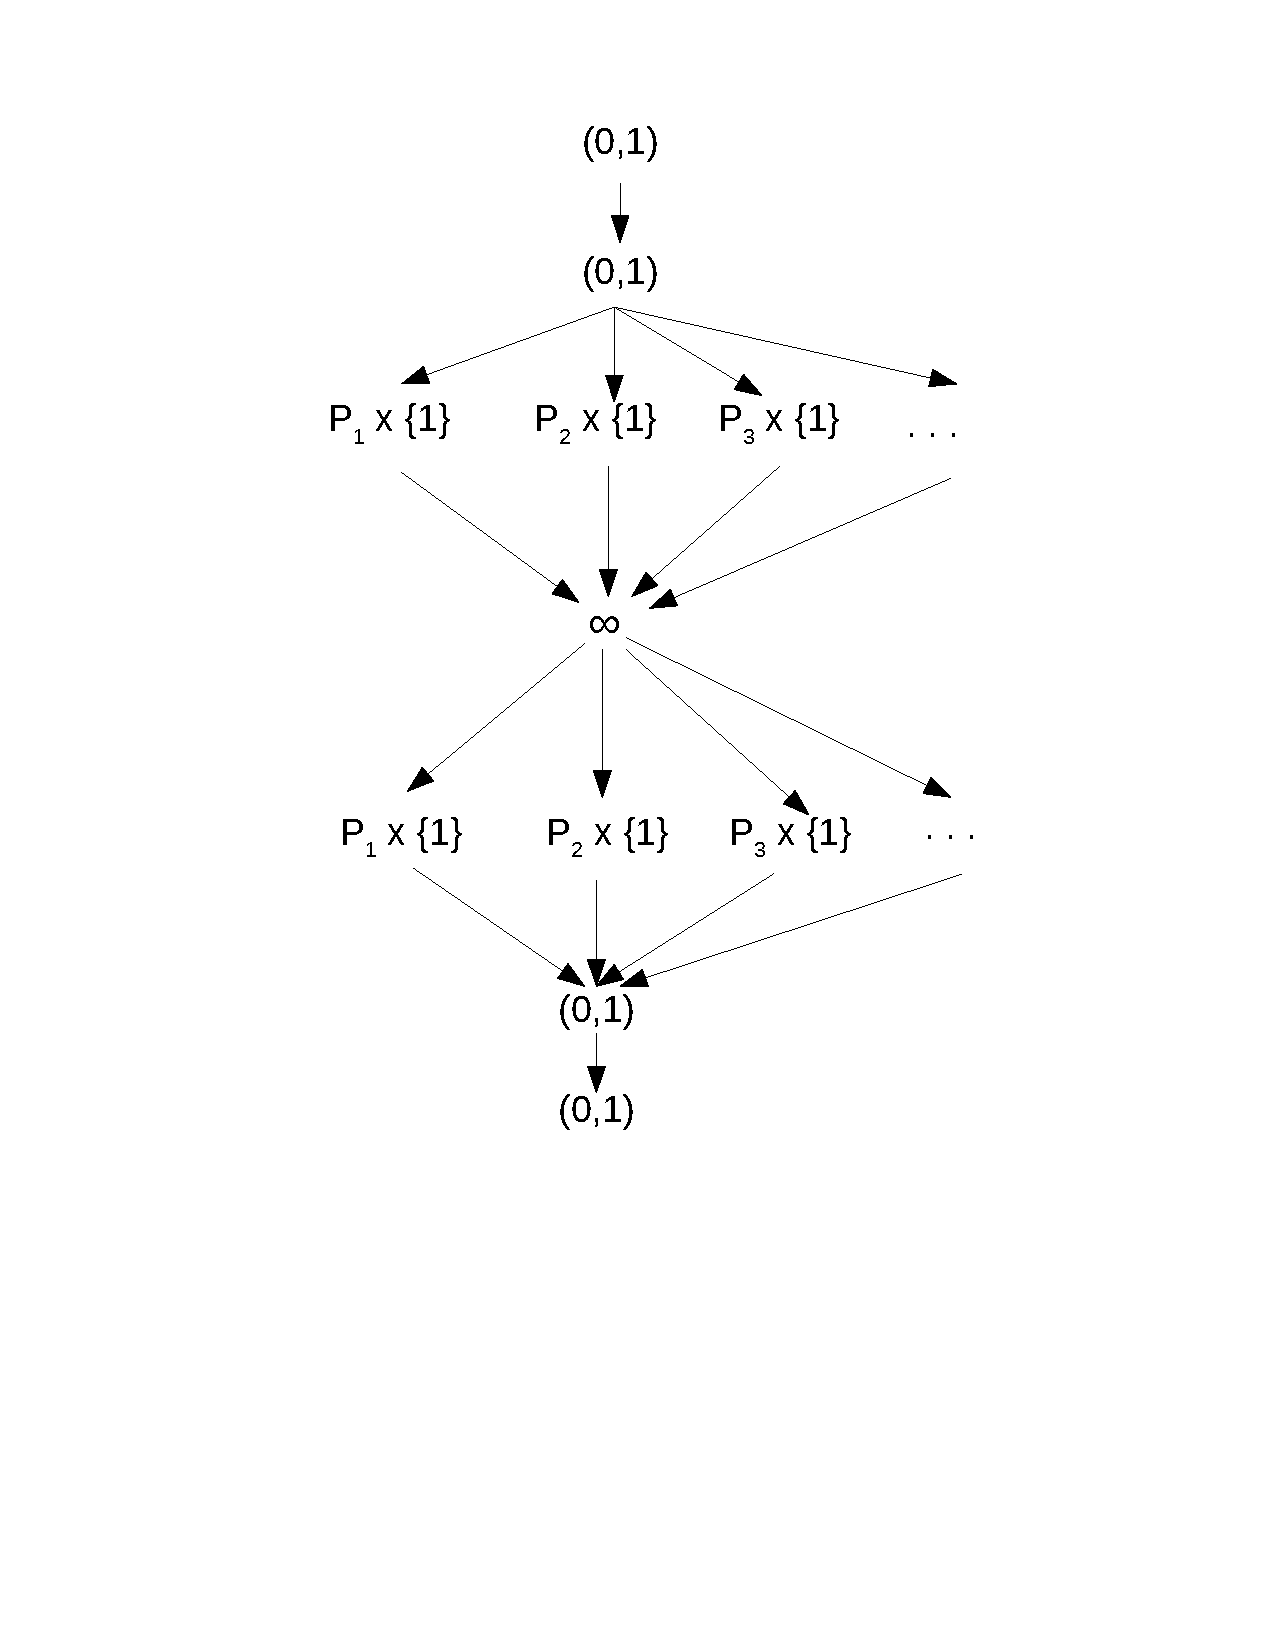
\includegraphics[scale=.4]{Ex3b.pdf}
\subsection*{c)}
for $(D,\sqsubseteq)$:\\
$d_1 \sqcup d2 =
\begin{cases}
d_1 \text{, if } d_2 \sqsubseteq d_1 \\
d_2 \text{, otherwise}
\end{cases}$\\\\
Note that $\sqsubseteq$ is total.\\\\
$d_1 \triangledown d2 =
\begin{cases}
\infty \text{, if } d_1,d_2 \in \mathbb{N} \times \{0\}, d_1 \neq d_2 \\
d_1 \sqcup d_2 \text{, otherwise}
\end{cases}$\\\\
This is a widening operator, because it basically "skips" the part of the lattice in which infinite ascending chains can occur.
Therefore every chain w.r.t the widening operator stabilizes.\\
for $(D,\preceq)$:\\
$d_1 \sqcup d2 =
\begin{cases}
d_1 \text{, if } d_2 \sqsubseteq d_1 \\
d_2 \text{, if } d_2 \sqsubseteq d_1 \\
\infty \text{, if } d_1,d_2 \in \mathbb{N}\times \{0\}, d_1 \not\preceq d_2, d_2 \not\preceq d_1 \\
(1,1) \text{, if } d_1,d_2 \in \mathbb{N}\times \{1\}, d_1 \not\preceq d_2, d_2 \not\preceq d_1
\end{cases}$\\\\

$d_1 \triangledown d2 =
\begin{cases}
\infty \text{, if } d_1 \in P_n \times \{0\}, d_2 \in P_n \times \{0\} \\
d_1 \sqcup d_2 \text{, otherwise}
\end{cases}$\\
Similar to above this widening operator "jumps upwards" in the lattice whenever it encounters two elements that are potentially part of an ascending chain.
And therefor the chains w.r.t this operator stabilizes because $\infty$ can not be a part of a non-stabilizing chain.
\section*{Exercise 4}

\end{document}
